% !TEX program = xelatex
% 本周（2026-10-12 至 2026-10-17）Daily Exercise List 回顾 · 讲解版
% 内容取自库内 10 - Daily Exercise Lists 的六份清单，以及对应的 25 篇习题笔记。
% 编译：xelatex -interaction=nonstopmode -halt-on-error <file>.tex（跑两遍以确定页数）
\documentclass[aspectratio=169,10pt,fontset=none]{ctexbeamer}

% ---------- 中英文字体 ----------
\usepackage{fontspec}
\setCJKmainfont{Microsoft YaHei}
\setCJKsansfont{Microsoft YaHei}

% ---------- 数学与图形 ----------
\usepackage{amsmath,amssymb}
\usepackage{booktabs}
\usepackage{array}
\usepackage{tikz}
\usetikzlibrary{arrows.meta,positioning,calc}

% ---------- 配色（沿用库内讲义配色） ----------
\definecolor{ink}{HTML}{1F3864}
\definecolor{accent}{HTML}{C00000}
\definecolor{gold}{HTML}{BF8F00}
\definecolor{greenink}{HTML}{2E6B2E}
\definecolor{paper}{HTML}{F5F7FA}

\usetheme{default}
\usecolortheme[named=ink]{structure}
\setbeamertemplate{navigation symbols}{}
\setbeamertemplate{itemize items}[circle]
\setbeamercolor{structure}{fg=ink}
\setbeamercolor{frametitle}{fg=ink}
\setbeamercolor{block title}{bg=ink!12,fg=ink}
\setbeamercolor{block body}{bg=ink!4,fg=black}
\setbeamercolor{block title alerted}{bg=accent!12,fg=accent}
\setbeamercolor{block body alerted}{bg=accent!4,fg=black}
\setbeamercolor{block title example}{bg=greenink!14,fg=greenink}
\setbeamercolor{block body example}{bg=greenink!5,fg=black}
\setbeamerfont{frametitle}{size=\large,series=\bfseries}
\setbeamerfont{footline}{size=\scriptsize}
\setbeamertemplate{frametitle}{\vskip3pt\insertframetitle\par\vskip1.5pt%
  \textcolor{accent}{\rule{\textwidth}{0.7pt}}\vskip-3pt}
\setbeamertemplate{footline}{%
  \hbox to \paperwidth{\hspace{8pt}%
    \textcolor{ink!55}{本周 Daily Exercise 回顾\ \ ·\ \ 10-12 -- 10-17\ \ ·\ \ 10-18 讲解版}\hfill
    \textcolor{ink!55}{\insertframenumber\,/\,\inserttotalframenumber}\hspace{9pt}}\vskip5pt}
\setbeamersize{text margin left=0.75cm,text margin right=0.75cm}
\setlength{\parindent}{0pt}
\setlength{\parskip}{2pt}
\AtBeginDocument{%
  \setlength{\abovedisplayskip}{3pt}\setlength{\belowdisplayskip}{3pt}%
  \setlength{\abovedisplayshortskip}{2pt}\setlength{\belowdisplayshortskip}{2pt}}

% 题号标记
\newcommand{\ex}[1]{\textcolor{accent}{\footnotesize\bfseries #1}}
\newcommand{\key}[1]{\textcolor{ink}{\bfseries #1}}
\newcommand{\starpt}{\textcolor{accent}{\bfseries$\ast$}}

\hypersetup{pdftitle={本周 Daily Exercise 回顾（2026-10-12 至 10-17，10-18 讲解版）},
  pdfsubject={Artin Algebra 2e, Ch. 7, Section 7.2-7.5: 25 exercises weekly review},
  pdfauthor={exercise\_abstract}}

\begin{document}

% ============================================================ 1 标题页
\begin{frame}[plain]
  \begin{tikzpicture}[remember picture,overlay]
    \fill[ink] (current page.north west) rectangle ([yshift=-4.7cm]current page.north east);
    \node[anchor=north west,text=white,font=\fontsize{26}{30}\selectfont\bfseries]
      at ([xshift=1.0cm,yshift=-0.92cm]current page.north west) {本周 Daily Exercise 回顾};
    \node[anchor=north west,text=white!90]
      at ([xshift=1.02cm,yshift=-2.10cm]current page.north west)
      {\large 覆盖 2026-10-12 -- 10-17（6 份清单，25 题）\quad·\quad 2026-10-18（周日）讲解版};
    \node[anchor=north west,text=white!75]
      at ([xshift=1.02cm,yshift=-2.92cm]current page.north west)
      {\normalsize Artin \textit{Algebra} 2e, Ch.~7, \S7.2--\S7.5\quad·\quad 群论 22 + 线性代数 3\quad·\quad 难度 6 / 11 / 8};
    \node[anchor=north east,text=white!60,font=\small]
      at ([xshift=-1.0cm,yshift=-0.92cm]current page.north east) {exercise\_abstract};
    \node[anchor=west,text=white!55,font=\tiny]
      at ([xshift=1.02cm,yshift=-4.42cm]current page.north west)
      {数据来源：\texttt{10 - Daily Exercise Lists} 的六份清单；结论取自 25 篇已核对习题笔记};
  \end{tikzpicture}
  \vspace*{4.85cm}
  \begin{columns}[T,onlytextwidth]
    \begin{column}{0.49\textwidth}
      \begin{block}{四条主线（按书序）}
        \scriptsize
        \begin{itemize}\setlength{\itemsep}{1pt}
          \item \key{\S7.2 共轭作用与类方程} \ex{LA198, G125--G129, LA199, LA200}
          \item \key{\S7.3 $p$-群与不动点} \ex{G195--G198}
          \item \key{\S7.4 群作用与多面体群} \ex{G199--G207}
          \item \key{\S7.5 对称群 $S_n$} \ex{G208--G211}
        \end{itemize}
      \end{block}
    \end{column}
    \begin{column}{0.47\textwidth}
      \begin{block}{这份讲解版的用法}
        \scriptsize
        \begin{itemize}\setlength{\itemsep}{1pt}
          \item 每道题给推导，不给"结论标签"；带 \starpt 的是要点
          \item 第 3 页是明天的讲解议程，第 26--27 页是全 25 题答案速查
          \item 第 30 页留了 8 道自测题，讲完当场做
        \end{itemize}
      \end{block}
    \end{column}
  \end{columns}
\end{frame}

% ============================================================ 2 本周概览
\begin{frame}[t]{一、本周概览：6 天、25 题、按书序推进}
  \begin{columns}[T,onlytextwidth]
    \begin{column}{0.58\textwidth}
      \centering
      \scriptsize
      \renewcommand{\arraystretch}{1.12}
      \begin{tabular}{@{}l r l@{}}
        \toprule
        日期 & 题数 & 题目（按清单顺序）\\
        \midrule
        10-12（一） & 10 & LA198, G125--G129, LA199, LA200, G195, G196\\
        10-13（二） & 3  & G197, G198, G199\\
        10-14（三） & 3  & G200, G201, G202\\
        10-15（四） & 3  & G203, G204, G205\\
        10-16（五） & 3  & G206, G207, G208\\
        10-17（六） & 3  & G209, G210, G211\\
        \midrule
        合计 & \textbf{25} & \S7.2 八题 + \S7.3 四题 + \S7.4 九题 + \S7.5 四题\\
        \bottomrule
      \end{tabular}
      \vspace{0.3em}

      \raggedright
      \begin{exampleblock}{\footnotesize 两个数据观察}
        \scriptsize
        \begin{itemize}\setlength{\itemsep}{1pt}
          \item \textbf{Random Review 本周 0 条}：25 题全部来自 Systematic Progress，明天讲完正好补上。
          \item \textbf{周一 10 题、之后每天 3 题}：\S7.2 一次扫完，后面按书序稳定推进，节奏适合今天一次讲完。
        \end{itemize}
      \end{exampleblock}
    \end{column}
    \begin{column}{0.40\textwidth}
      \centering
      \begin{tikzpicture}[x=0.58cm,y=0.37cm]
        \foreach \d/\n [count=\i] in {一/10, 二/3, 三/3, 四/3, 五/3, 六/3}{
          \fill[ink!75] (\i-0.28,0) rectangle (\i+0.28,\n);
          \node[above,font=\tiny,text=ink] at (\i,\n) {\n};
          \node[below,font=\tiny,text=ink!80] at (\i,0) {\d};
        }
        \draw[ink!45] (0.35,0) -- (6.65,0);
        \node[right,font=\tiny,text=accent] at (6.75,4) {25 题};
        \node[below,font=\tiny,text=ink!60] at (3.5,-1.0) {每日题量};
      \end{tikzpicture}

      \vspace{0.3em}
      \begin{block}{\footnotesize 难度与来源}
        \scriptsize
        入门 6 · 中等 11 · 高级 8。\\[1pt]
        Artin 2e Ch.~7 \S7.2--\S7.5，印刷 pp.~221--223 / PDF pp.~233--235；\ex{G198}、\ex{G208} 另含 Lang I.35、I.38。
      \end{block}
    \end{column}
  \end{columns}
\end{frame}

% ============================================================ 3 讲解议程
\begin{frame}[t]{二、明天（10-18）怎么讲：80 分钟议程}
  \centering
  \footnotesize
  \renewcommand{\arraystretch}{1.22}
  \begin{tabular}{@{}l l r@{}}
    \toprule
    时间 & 内容 & 页码\\
    \midrule
    8 分钟  & 框架：轨道--稳定化子、类方程、正规子群判别 + 两条小引理 & 4--5\\
    22 分钟 & \S7.2 八题：矩阵中心化子、类方程案例、共轭判定 & 6--12\\
    12 分钟 & \S7.3 四题：不动点定理、$p^3$、8 阶群分类 & 13--15\\
    18 分钟 & \S7.4 九题：$T/O/I$ 的类方程与正规子群、群作用 & 16--22\\
    12 分钟 & \S7.5 四题：轮换型中心化子、$S_n$ 的生成元 & 23--25\\
    8 分钟  & 收尾：答案速查表、六张方法卡、易错点 + 当场自测 & 26--30\\
    \bottomrule
  \end{tabular}

  \vspace{0.5em}
  \raggedright
  \begin{columns}[T,onlytextwidth]
    \begin{column}{0.55\textwidth}
      \begin{block}{\footnotesize 讲法建议}
        \scriptsize
        \begin{itemize}\setlength{\itemsep}{1pt}
          \item 每题先让学生说"该算哪个量"，再翻到推导页
          \item 类方程的三步：数类大小 → 拼正规子群 → 检查整除性
          \item $T/O/I$ 用一张几何图带过轴结构与置换表示，不要逐题重画
        \end{itemize}
      \end{block}
    \end{column}
    \begin{column}{0.43\textwidth}
      \begin{alertblock}{\footnotesize 一个变数：10-18 的清单}
        \scriptsize
        周日清单在 0:00 生成，若明天要连当天的 3 题一起讲，讲前按 \S7.5 的结构补一页（题面 + 结论 + 速查表补行），页码顺延即可。
      \end{alertblock}
    \end{column}
  \end{columns}
  \vspace{0.3em}

  {\scriptsize\color{ink!70} 时间可按实际压缩：若只剩 60 分钟，把 \S7.4 压到 12 分钟、速查表（26--27 页）留作课后阅读；若 10-18 的清单已经生成，先讲当天 3 题再回到本片。}
\end{frame}

% ============================================================ 4 框架：三条公式
\begin{frame}[t]{三、框架 1/2：三条公式与它们的证明}
  \begin{block}{1. 轨道--稳定化子 $\Rightarrow$ 类大小公式}
    \footnotesize
    共轭作用 $x^g=gxg^{-1}$ 的轨道与稳定化子分别是 $C(x)$ 与 $Z_G(x)$，故
    \[ |C(x)|=[G:Z_G(x)]\qquad\Longleftrightarrow\qquad |G|=|C(x)|\cdot|Z_G(x)|. \]
  \end{block}
  \begin{block}{2. 类方程}
    \footnotesize
    按共轭类切开 $G$，中心的类都是单点，其余类大小是 $[G:Z_G(x_i)]$：
    \[ |G|=|Z(G)|+\sum_{i}\,[G:Z_G(x_i)]. \]
  \end{block}
  \begin{block}{3. 正规子群 $=$ 含 $1$ 的若干共轭类之并}
    \footnotesize
    $N\trianglelefteq G$ $\iff$ $N$ 对共轭封闭 $\iff$ $N$ 是类之并，于是 $|N|$ 等于 $1$ 加若干类大小，且 $|N|\mid|G|$。
  \end{block}
\end{frame}

% ============================================================ 5 两条引理
\begin{frame}[t]{三、框架 2/2：两条反复调用的小引理}
  \begin{columns}[T,onlytextwidth]
    \begin{column}{0.49\textwidth}
      \begin{alertblock}{\footnotesize 引理 A（G126）$5$ 阶正规子群必中心}
        \scriptsize
        设 $N\trianglelefteq G$，$|N|=5$，$|G|$ 为奇数。则 $N\subseteq Z(G)$。\\[2pt]
        \textbf{证明.} $|N|=5$ 素 $\Rightarrow N\cong C_5$，$|\operatorname{Aut}(C_5)|=\varphi(5)=4$。共轭给出同态
        \[ \theta:G\to\operatorname{Aut}(N),\qquad |\operatorname{im}\theta|\mid|G|,\quad |\operatorname{im}\theta|\mid4. \]
        因 $|G|$ 奇，$|\operatorname{im}\theta|=1$，即 $gng^{-1}=n$。$\square$\\[2pt]
        \key{奇阶不可省}：$G=C_5\rtimes C_4$（阶 20）中 $C_5\trianglelefteq G$，但 $C_4$ 在其上作非平凡自同构，$C_5$ 不中心。
      \end{alertblock}
    \end{column}
    \begin{column}{0.49\textwidth}
      \begin{alertblock}{\footnotesize 引理 B（G196）$G/Z(G)$ 循环 $\Rightarrow$ $G$ 交换}
        \scriptsize
        设 $G/Z(G)=\langle aZ\rangle$。任意 $x,y\in G$ 可写
        \[ x=a^m z,\qquad y=a^n w,\qquad z,w\in Z(G). \]
        则 $xy=a^{m+n}zw=a^{n+m}wz=yx$，故 $G$ 交换，$G=Z(G)$。$\square$\\[3pt]
        \key{本周三次调用：}
        \begin{itemize}\setlength{\itemsep}{0pt}
          \item \ex{G197}：排除 $|Z|=p^2$（否则 $G/Z$ 是 $p$ 阶，循环）；
          \item \ex{G207}：$C/Z(C)$ 是循环商，故 $C$ 交换；
          \item \ex{LA199} 的对照：$SL_2(\mathbb F_3)/\{\pm I\}$ 不是循环群，所以不矛盾。
        \end{itemize}
      \end{alertblock}
    \end{column}
  \end{columns}
  \footnotesize\color{ink!80}
  \starpt 两条引理一个管"正规子群能有多大"，一个管"中心能有多小"，正好夹住类方程里 $|Z(G)|$ 的可能值。
\end{frame}

% ============================================================ 6 LA198 1/2
\begin{frame}[t]{四、\S7.2 精算 1/8：LA198 五个矩阵的中心化子（上）}
  \centering
  \begin{block}{\footnotesize 总表：解 $PA=AP$，$P\in GL_3(\mathbb R)$}
    \scriptsize
    \renewcommand{\arraystretch}{1.22}
    \begin{tabular}{@{}l l c@{}}
      \toprule
      矩阵 & $Z_{GL_3(\mathbb R)}(A)$ & $\dim$\\
      \midrule
      $A_1$（特征值 $1,2,3$） & $\operatorname{diag}(a,b,c)$，$abc\ne0$ & 3\\
      $A_2$（特征值 $1,1,2$） & $\begin{pmatrix}B&0\\0&c\end{pmatrix}$，$B\in GL_2(\mathbb R)$，$c\ne0$ & 5\\
      $A_3=I+E_{12}$ & $\begin{pmatrix}a&b&c\\0&a&0\\0&h&k\end{pmatrix}$，$ak\ne0$ & 5\\
      $A_4=J_3(1)$ & $aI+bN+cN^2$，$a\ne0$ & 3\\
      $A_5$（交换 $e_1,e_3$） & $a_{ij}=a_{4-i,\,4-j}$（中心对称） & 5\\
      \bottomrule
    \end{tabular}
  \end{block}
  \raggedright
  \begin{block}{前两个怎么来的}
    \scriptsize
    \textbf{$A_1$：}三个特征值互异，每个特征空间都是 1 维。$P$ 与 $A_1$ 交换就必须把每条特征线送到自身（否则 $P$ 会把特征向量拉到别的特征空间，$A_1P=PA_1$ 在特征值上矛盾），于是 $P$ 只能对角。\\
    \textbf{$A_2$：}$1$ 的特征空间 2 维、$2$ 的特征空间 1 维；两个特征空间互异，$P$ 必须同时保持它们，于是 $P$ 分块对角，左上任意可逆 $2\times2$，右下非零标量。
  \end{block}
\end{frame}

% ============================================================ 7 LA198 2/2
\begin{frame}[t]{四、\S7.2 精算 1/8：LA198 五个矩阵的中心化子（下）}
  \begin{columns}[T,onlytextwidth]
    \begin{column}{0.49\textwidth}
      \begin{block}{\footnotesize $A_3=I+E_{12}$：直接解方程}
        \scriptsize
        记 $P=(p_{ij})$。$PA_3=A_3P$ 等价于
        \[ PE_{12}=E_{12}P. \]
        左边只有第 2 列，等于 $P$ 的第 1 列 $(p_{11},p_{21},p_{31})^{\mathsf T}$；右边只有第 1 行，等于 $P$ 的第 2 行 $(p_{21},p_{22},p_{23})$。比较得
        \[ (0,p_{11},0)=(p_{21},p_{22},p_{23}),\qquad p_{31}=0, \]
        即 $p_{21}=p_{23}=p_{31}=0$、$p_{22}=p_{11}$，故 $P$ 形如表中矩阵，$\det P=a^2k$。
      \end{block}
      \begin{block}{\footnotesize $A_4=J_3(1)$：与幂零部分交换}
        \scriptsize
        $A_4=I+N$，$N=E_{12}+E_{23}$，$N^2=E_{13}$，$N^3=0$。$P$ 与 $I+N$ 交换 $\iff$ $PN=NP$，而所有与 $N$ 交换的矩阵恰是 $N$ 的多项式：
        \[ Z(A_4)=\{aI+bN+cN^2:a\ne0\}. \]
      \end{block}
    \end{column}
    \begin{column}{0.49\textwidth}
      \begin{block}{\footnotesize $A_5$：置换型，保持对称结构}
        \scriptsize
        $A_5$ 交换 $e_1,e_3$、固定 $e_2$。$P$ 与它交换 $\iff$ $P$ 的条目满足中心对称 $p_{ij}=p_{4-i,4-j}$：
        \[ Z(A_5)=\left\{\begin{pmatrix}a&b&c\\d&e&d\\c&b&a\end{pmatrix}:\det\ne0\right\}. \]
      \end{block}
      \begin{block}{\footnotesize 解 $PA=AP$ 的四条套路}
        \scriptsize
        \begin{enumerate}\setlength{\itemsep}{1pt}
          \item 特征值互异 $\Rightarrow$ 对角（$A_1$）。
          \item 重特征值 $\Rightarrow$ 保持广义特征空间，分块（$A_2$）。
          \item 不可对角化 $\Rightarrow$ 与幂零部分交换，只剩多项式（$A_4$）。
          \item 置换型 $\Rightarrow$ 检查结构对称（$A_5$、以及 \ex{LA200} 的 $d$ 参数）。
        \end{enumerate}
        \key{提醒}：换成 $SL_3$ 或 $SL_2$ 时还要把 $\det P$ 归一，这正是 \ex{LA200} 变难的原因。
      \end{block}
    \end{column}
  \end{columns}
\end{frame}

% ============================================================ 8 G125
\begin{frame}[t]{四、\S7.2 精算 2/8：G125 至多三个共轭类的群}
  \begin{block}{分类：$\{1\},\ C_2,\ C_3,\ S_3$}
    \small
    记共轭类数为 $r\le 3$，逐个排除。
  \end{block}
  \begin{columns}[T,onlytextwidth]
    \begin{column}{0.49\textwidth}
      \begin{exampleblock}{\footnotesize $r=1,2$ 与 $r=3$ 的交换情形}
        \scriptsize
        $r=1$：$G$ 只有一个类 $\Rightarrow G=\{1\}$。\\
        $r=2$：$|G|=1+a$，$a$ 是某个中心化子的指数，故 $a\mid|G|$，但 $a=|G|-1\mid1$ $\Rightarrow a=1$，$|G|=2$，$G=C_2$。\\
        $r=3$ 且交换：每个类单点 $\Rightarrow |G|=3$，$G=C_3$。
      \end{exampleblock}
      \begin{exampleblock}{\footnotesize $r=3$ 非交换：中心只能是 $1$}
        \scriptsize
        若 $|Z|=2$，类方程 $|G|=1+1+a$，$a=|G|-2$，由 $a\mid|G|$ 得 $a\mid2$，于是 $|G|\le4$，与"三个类且非交换"矛盾。\\
        所以 $Z=1$，$|G|=1+a+b$，$1<a\le b$，且 $a,b$ 都整除 $|G|$。
      \end{exampleblock}
    \end{column}
    \begin{column}{0.49\textwidth}
      \begin{alertblock}{\footnotesize 非交换情形的整除链}
        \scriptsize
        \begin{enumerate}\setlength{\itemsep}{2pt}
          \item $a=b$ 不可能：若 $a=b$，则 $a\mid|G|=1+2a$ $\Rightarrow a\mid1$，与 $a>1$ 矛盾。
          \item 故 $b>a$，又 $b\mid1+a$，于是 $a+1\le b\le a+1$，即 $b=a+1$。
          \item 代回 $|G|=2a+2$；再由 $a\mid|G|$ 得 $a\mid2$，故 $a=2$，$b=3$，$|G|=6$。
          \item 6 阶非交换群唯一：$S_3$，类方程 $6=1+2+3$。
        \end{enumerate}
        \starpt 这条链只用"类大小整除群阶"，没有用任何 Sylow 工具。
      \end{alertblock}
    \end{column}
  \end{columns}
\end{frame}

% ============================================================ 9 G127
\begin{frame}[t]{四、\S7.2 精算 3/8：G127 类方程 $1+4+5+5+5$}
  \begin{block}{已知：$|G|=20$，$Z(G)=1$，类大小 $1,4,5,5,5$}
    \scriptsize
    问题有(a)(b)两问，答案正好相反：$5$ 阶子群存在且\textbf{正规}；$4$ 阶子群存在但\textbf{不正规}。
  \end{block}
  \begin{columns}[T,onlytextwidth]
    \begin{column}{0.49\textwidth}
      \begin{exampleblock}{\footnotesize (a) 阶 5：取 4 元类元素的中心化子}
        \scriptsize
        设 $x$ 在 $|C(x)|=4$ 的类里，则 $H:=Z_G(x)$ 满足
        \[ |H|=|G|/|C(x)|=20/4=5, \]
        所以 $H$ 是 5 阶子群。任取 $1\ne h\in H$，有 $H\subseteq Z_G(h)$，故
        \[ |C(h)|=20/|Z_G(h)|\le 20/5=4. \]
        类方程里 $\le4$ 的非中心类只有 $4$ 这一项，于是 $H\setminus\{1\}=C(x)$ 恰是一个类，$H=\{1\}\cup C(x)$ 是类之并，故 $H\trianglelefteq G$。
      \end{exampleblock}
    \end{column}
    \begin{column}{0.49\textwidth}
      \begin{alertblock}{\footnotesize (b) 阶 4：存在，但不可能是类之并}
        \scriptsize
        设 $y$ 在 $|C(y)|=5$ 的类里，则 $K:=Z_G(y)$ 满足 $|K|=20/5=4$，所以 4 阶子群存在。
        若它正规，则 $K$ 必是含 $1$ 的类之并，$|K|=4$ 要写成
        \[ 1+\varepsilon_4\cdot4+\varepsilon_5\cdot5+\varepsilon_5'\cdot5+\varepsilon_5''\cdot5, \]
        其中 $\varepsilon_\bullet\in\{0,1\}$。逐个检查：$1$、$1+4=5$、$1+5=6$、$1+4+5=10$、$\dots$，没有 $4$。故 $K$ 不正规。
      \end{alertblock}
      \footnotesize\color{ink!80}
      \starpt 存在性问"中心化子多大"，正规性问"能否写成类之和"，两者互不蕴含。
    \end{column}
  \end{columns}
\end{frame}

% ============================================================ 10 LA199
\begin{frame}[t]{四、\S7.2 精算 4/8：LA199 $SL_2(\mathbb F_3)$ 的七类}
  \begin{block}{$|SL_2(\mathbb F_3)|=3(3^2-1)=24$，七个共轭类}
    \scriptsize
    \renewcommand{\arraystretch}{1.15}
    \begin{tabular}{@{}l l c c@{}}
      \toprule
      代表元 & 说明 & $|Z|$ & $|C|$\\
      \midrule
      $I,\ -I$ & 中心元（$\det=1$ 的标量只有 $\pm1$） & 24 & 1, 1\\
      $\begin{pmatrix}1&a\\0&1\end{pmatrix}$ 及其负，$a=\pm1$ & $U_1,U_{-1}$ 及其负，共四类 & 6 & 4\\
      $\begin{pmatrix}0&-1\\1&0\end{pmatrix}$ & 迹 $0$ 的元素 & 4 & 6\\
      \bottomrule
    \end{tabular}\\[1pt]
    合计：$24=1+1+4+4+4+4+6$。
  \end{block}
  \begin{columns}[T,onlytextwidth]
    \begin{column}{0.49\textwidth}
      \begin{block}{\footnotesize 中心化子怎么算}
        \scriptsize
        $U_a$ 在 $SL_2$ 中的中心化子是 $\left\{\begin{pmatrix}s&t\\0&s\end{pmatrix}:s=\pm1,\ t\in\mathbb F_3\right\}$，共 $6$ 个，故类大小 $24/6=4$。迹 $0$ 的 $A$ 与 $P$ 交换 $\iff P\in\{\pm I,\pm A\}$，阶 $4$。
      \end{block}
    \end{column}
    \begin{column}{0.49\textwidth}
      \begin{alertblock}{\footnotesize $U_1$ 与 $U_{-1}$ 为什么不共轭}
        \scriptsize
        共轭保持公共特征线 $e_1$，故 $P$ 上三角：$P=\begin{pmatrix}\lambda&\mu\\0&\lambda^{-1}\end{pmatrix}$，且
        \[ P U_1 P^{-1}=U_{\lambda^2}. \]
        $\mathbb F_3^\times$ 中 $\lambda^2=1$，只能得到 $U_1$；$GL_2$ 里 $\lambda$ 可任取，两者才共轭。
      \end{alertblock}
    \end{column}
  \end{columns}
\end{frame}

% ============================================================ 11 G128/G129
\begin{frame}[t]{四、\S7.2 精算 5/8：G128 满射与 G129 $pq$ 阶群}
  \begin{columns}[T,onlytextwidth]
    \begin{column}{0.49\textwidth}
      \begin{block}{\footnotesize G128：$\varphi(C)=C'$ 且 $|C'|\mid|C|$}
        \scriptsize
        \textbf{映满。} 对 $g\in G$：
        \[ \varphi(gxg^{-1})=\varphi(g)\varphi(x)\varphi(g)^{-1}, \]
        故 $\varphi(C)\subseteq C'$；反之 $C'$ 的任一元素为 $g'\varphi(x)g'^{-1}$，由满射写 $g'=\varphi(g)$，它是 $gxg^{-1}\in C$ 的像。\\
        \textbf{整除。} 令 $H=\varphi^{-1}\bigl(Z_{G'}(\varphi(x))\bigr)$，则 $Z_G(x)\le H$，且
        \[ |C'|=[G':Z_{G'}(\varphi(x))]=[G:H], \]
        \[ |C|=[G:Z_G(x)]=[G:H]\,[H:Z_G(x)], \]
        故 $|C'|\mid|C|$。
      \end{block}
      \footnotesize\color{ink!80}
      注：映满不要求有限；整除那条用了有限性。
    \end{column}
    \begin{column}{0.49\textwidth}
      \begin{alertblock}{\footnotesize G129：$|G|=pq$ 必有 $p$ 阶元}
        \scriptsize
        $p=q$ 时非单位元的阶是 $p$ 或 $p^2$，后者取其 $p$ 次幂即可。设 $p\ne q$，反设无 $p$ 阶元。\\[1pt]
        \textbf{情形 1：$Z(G)\ne1$。} 取 $1\ne z\in Z$。$z$ 的阶不能是 $p$ 或 $pq$，否则有 $p$ 阶元，故 $|z|=q$。于是 $|G/\langle z\rangle|=p$。对 $x\notin\langle z\rangle$，其像的阶为 $p$，故 $x^p\in\langle z\rangle$；$x$ 的阶不能是 $q$（像的阶同时整除 $p,q$），只能是 $pq$，于是 $x^q$ 阶为 $p$，矛盾。\\[1pt]
        \textbf{情形 2：$Z(G)=1$。} 每个非单位元阶为 $q$（$pq$ 阶会给 $p$ 阶元）。其中心化子含 $\langle x\rangle$ 且真，故阶为 $q$，从而每个非中心类大小 $p$：
        \[ pq=1+kp, \]
        模 $p$ 矛盾。
      \end{alertblock}
    \end{column}
  \end{columns}
\end{frame}

% ============================================================ 12 LA200
\begin{frame}[t]{四、\S7.2 精算 6/8：LA200 $GL_2$ 与 $SL_2$ 中的共轭}
  \begin{columns}[T,onlytextwidth]
    \begin{column}{0.50\textwidth}
      \begin{block}{\footnotesize 解 $PA_d=B_dP$}
        \scriptsize
        \[ A_d=\begin{pmatrix}0&1\\-1&d\end{pmatrix},\qquad B_d=\begin{pmatrix}0&-1\\1&d\end{pmatrix},\qquad P=\begin{pmatrix}a&b\\c&e\end{pmatrix}. \]
        逐项比较 $PA_d=B_dP$：
        \[ c=b,\qquad e=-a-db, \]
        故所有 intertwiner 是
        \[ P=\begin{pmatrix}a&b\\b&-a-db\end{pmatrix},\qquad \det P=-(a^2+dab+b^2). \]
      \end{block}
      \begin{exampleblock}{\footnotesize $GL_2(\mathbb R)$：恒共轭}
        \scriptsize
        取 $(a,b)=(1,0)$ 得 $P=\operatorname{diag}(1,-1)$，$\det P=-1\ne0$，与 $d$ 无关。
      \end{exampleblock}
    \end{column}
    \begin{column}{0.48\textwidth}
      \begin{alertblock}{\footnotesize $SL_2(\mathbb R)$：当且仅当 $|d|>2$}
        \scriptsize
        需要 $\det P=1$，即二次型
        \[ q(a,b)=a^2+dab+b^2=-1. \]
        $q$ 的判别式为 $d^2-4$：
        \begin{itemize}\setlength{\itemsep}{1pt}
          \item $|d|\le2$：$q$ 半正定（$d=\pm2$ 时分别是 $(a\pm b)^2$），取不到负值；
          \item $|d|>2$：$q$ 不定，在 $\mathbb R^2$ 上取到所有实数，特别地 $-1$。
        \end{itemize}
      \end{alertblock}
      \begin{alertblock}{\footnotesize 题面注记}
        \scriptsize
        矩阵是 $2\times2$，印的却是 $GL_n/SL_n$。笔记保留原题并标 \texttt{Source issue}，再按 $n=2$ 解；不要悄悄把题面改成 $GL_2$。
      \end{alertblock}
    \end{column}
  \end{columns}
\end{frame}

% ============================================================ 13 不动点定理
\begin{frame}[t]{五、\S7.3 精算 1/4：不动点定理（G195）}
  \begin{columns}[T,onlytextwidth]
    \begin{column}{0.53\textwidth}
      \begin{block}{定理（Artin 7.3.2）}
        \small
        有限 $p$-群 $G$ 作用在有限集 $S$ 上，$S^G$ 为不动点集，则
        \[ |S|\equiv|S^G|\pmod p,\qquad p\nmid|S|\ \Rightarrow\ S^G\ne\varnothing. \]
      \end{block}
      \begin{block}{\footnotesize 证明（只用轨道--稳定化子）}
        \scriptsize
        把 $S$ 分成轨道。轨道大小 $=[G:G_s]$ 整除 $|G|$，因而是 $p$ 的幂。
        单点轨道就是不动点，恰好 $|S^G|$ 个；其余轨道大小都被 $p$ 整除。相加：
        \[ |S|=|S^G|+\sum_{|Gs|>1}|Gs|\equiv|S^G|\pmod p. \]
        若 $p\nmid|S|$，则 $|S^G|\not\equiv0$，特别地非空。$\square$
      \end{block}
      \begin{alertblock}{\footnotesize 推论：$p$-群中心非平凡}
        \scriptsize
        取共轭作用 $S=G$，不动点集就是 $Z(G)$，于是 $|Z(G)|\equiv|G|\equiv0\pmod p$，而 $1\in Z(G)$，故 $|Z(G)|\ge p$。
      \end{alertblock}
    \end{column}
    \begin{column}{0.45\textwidth}
      \centering
      \begin{tikzpicture}[x=0.80cm,y=0.80cm]
        \foreach \i in {0,1,2}{\fill[greenink!35] (\i*0.88,0) rectangle ++(0.78,0.78);}
        \node[font=\tiny,text=greenink,anchor=north] at (0.88,-0.12) {不动点（单点轨道）};
        \fill[ink!22] (3.05,0) rectangle ++(1.20,0.78); \node[font=\tiny] at (3.65,0.39) {$p$};
        \fill[ink!14] (4.35,0) rectangle ++(1.20,0.78); \node[font=\tiny] at (4.95,0.39) {$p$};
        \fill[gold!28] (5.65,0) rectangle ++(1.80,0.78); \node[font=\tiny] at (6.55,0.39) {$p^2$};
        \node[font=\tiny,text=ink!70,anchor=north] at (4.9,-0.12) {其余轨道：大小是 $p$ 的幂};
      \end{tikzpicture}

      \vspace{0.4em}
      \raggedright
      \begin{block}{\footnotesize 本周哪里用到了它}
        \scriptsize
        \begin{itemize}\setlength{\itemsep}{1pt}
          \item \ex{G195}：定理本身的证明；
          \item \ex{G197}：$|Z|\equiv|G|\equiv0\pmod p$，先把中心"撑"到至少 $p$ 阶；
          \item 复用的技巧：$p\nmid|S|$ 时断言"必有不动点"，是后面 Sylow 章节的预备动作，本周还没真正用到。
        \end{itemize}
      \end{block}
    \end{column}
  \end{columns}
\end{frame}

% ============================================================ 14 G197
\begin{frame}[t]{五、\S7.3 精算 2/4：G197 非交换 $p^3$ 的三问}
  \begin{columns}[T,onlytextwidth]
    \begin{column}{0.50\textwidth}
      \begin{block}{\footnotesize (a) 中心的阶只能是 $p$}
        \scriptsize
        对共轭作用用不动点定理：$|Z|\equiv|G|=p^3\equiv0\pmod p$，故 $p\mid|Z|$，即 $|Z|\in\{p,p^2,p^3\}$。
        $|Z|=p^3$ 表示 $G$ 交换，排除；若 $|Z|=p^2$，则 $|G/Z|=p$ 是素数阶群，必循环，由引理 B 得 $G$ 交换，排除。故 $|Z|=p$。
      \end{block}
      \begin{block}{\footnotesize (b)(c) 中心化子与类方程}
        \scriptsize
        取 $x\notin Z$。则 $Z\subsetneq Z(x)\subsetneq G$，三者的阶都是 $p$ 的幂，所以 $|Z(x)|=p^2$。
        于是每个非中心类的大小为
        \[ [G:Z(x)]=p^3/p^2=p. \]
        非中心元共 $p^3-p$ 个，故非中心类有 $(p^3-p)/p=p^2-1$ 个，即
        \[ p^3=p+(p^2-1)\,p. \]
      \end{block}
    \end{column}
    \begin{column}{0.48\textwidth}
      \begin{exampleblock}{\footnotesize 用 $p=2$ 对账}
        \scriptsize
        $p=2$ 时类方程为
        \[ 8=2+3\cdot2=1+1+2+2+2, \]
        正是 $D_4$ 与 $Q_8$ 的类方程（中心 2 个元素、三个 2 元类）。\\
        反过来，这个方程也说明"非交换 8 阶群"的类结构被 $p^3$ 一般公式完全锁死。
      \end{exampleblock}
      \begin{alertblock}{\footnotesize 关键推理顺序（别记反）}
        \scriptsize
        \begin{enumerate}\setlength{\itemsep}{1pt}
          \item 不动点定理只给出 $p\mid|Z|$；
          \item 引理 B 排掉 $|Z|=p^2$；
          \item 剩下 $|Z|=p$ 才推出中心化子 $p^2$；
          \item 中心化子大小 $\Rightarrow$ 类大小 $\Rightarrow$ 类数。
        \end{enumerate}
        若把第 2 步漏掉，会得到"$|Z|$ 可以是 $p^2$"的错误结论。
      \end{alertblock}
    \end{column}
  \end{columns}
\end{frame}

% ============================================================ 15 G198
\begin{frame}[t]{五、\S7.3 精算 3/4：G198 八阶群的完整分类}
  \begin{columns}[T,onlytextwidth]
    \begin{column}{0.50\textwidth}
      \begin{block}{\footnotesize 交换情形：三个群}
        \scriptsize
        阶 8 的交换群由分拆 $3$ 决定（对应循环因子分解）：
        \[ C_8,\qquad C_4\times C_2,\qquad C_2^3. \]
        也可按"是否有 8 阶元 / 4 阶元个数"直接分类。
      \end{block}
      \begin{block}{\footnotesize 非交换情形：必有 4 阶元}
        \scriptsize
        若所有非单位元的阶都是 2，则 $(xy)^2=1$，于是
        \[ xy=(xy)^{-1}=y^{-1}x^{-1}=yx, \]
        群就交换了，矛盾。故存在 4 阶元 $a$。
      \end{block}
      \begin{exampleblock}{\footnotesize 两种可能}
        \scriptsize
        $\langle a\rangle$ 指数 2，必正规。取 $b\notin\langle a\rangle$。共轭诱导 $\operatorname{Aut}(C_4)$ 的自同构必须非平凡，故 $bab^{-1}=a^{-1}$。\\
        又 $b^2\in\langle a\rangle$ 且与 $b$ 交换，代入得 $a^{2k}=1$，故
        \[ b^2=1\ \Rightarrow\ D_4;\qquad b^2=a^2\ \Rightarrow\ Q_8. \]
      \end{exampleblock}
    \end{column}
    \begin{column}{0.48\textwidth}
      \centering
      \begin{block}{\footnotesize 五个群的区分}
        \scriptsize
        \renewcommand{\arraystretch}{1.18}
        \begin{tabular}{@{}l l l@{}}
          \toprule
          群 & 类方程 & 元素阶剖面\\
          \midrule
          $C_8$ & $1+\cdots+1$ & $1,2,4,8$\\
          $C_4\times C_2$ & $1+\cdots+1$ & $1,2,4$\\
          $C_2^3$ & $1+\cdots+1$ & $1,2$\\
          $D_4$ & $1+1+2+2+2$ & 5 个 2 阶、2 个 4 阶\\
          $Q_8$ & $1+1+2+2+2$ & 1 个 2 阶、6 个 4 阶\\
          \bottomrule
        \end{tabular}
      \end{block}
      \footnotesize\color{ink!80}
      \starpt $D_4$ 与 $Q_8$ 的类方程完全一样、中心同为 2 阶，必须用元素阶剖面（或子群结构）才能分开——这是本周"类方程不是完全同构不变量"的唯一例子。
    \end{column}
  \end{columns}
\end{frame}

% ============================================================ 16 T/O/I 总览
\begin{frame}[t]{六、\S7.4 精算 1/9：$T$、$O$、$I$ 的旋转结构与置换表示}
  \centering
  \begin{block}{\footnotesize 三个旋转群的"身份证"}
    \scriptsize
    \renewcommand{\arraystretch}{1.3}
    \begin{tabular}{@{}l l l l c l@{}}
      \toprule
      群 & 几何载体 & 忠实的低次作用 & 旋转轴 & 阶 & 同构\\
      \midrule
      $T$ & 正四面体 & 4 个顶点 & 4 条三重 $+\ 3$ 条二重 & 12 & $A_4$\\
      $O$ & 立方体 / 正八面体 & 4 条体对角线 & 3 条四重 $+\ 4$ 条三重 $+\ 6$ 条二重 & 24 & $S_4$\\
      $I$ & 正十二面体 / 正二十面体 & 5 个内接立方体 & 6 条五重 $+\ 10$ 条三重 $+\ 15$ 条二重 & 60 & $A_5$\\
      \bottomrule
    \end{tabular}
  \end{block}
  \raggedright
  \begin{columns}[T,onlytextwidth]
    \begin{column}{0.49\textwidth}
      \begin{block}{\footnotesize 表怎么用}
        \scriptsize
        \begin{itemize}\setlength{\itemsep}{1pt}
          \item 旋转轴的重数直接给出共轭类：同重数的轴上的旋转（同角度）共轭；
          \item 2 重轴上的半转 = 双对换/对换，是类方程里的大类；
          \item 3 重轴给 3-轮换，5 重轴给 5-轮换，且 $A_5$ 里 5-轮换分成两族。
        \end{itemize}
      \end{block}
    \end{column}
    \begin{column}{0.49\textwidth}
      \begin{exampleblock}{\footnotesize 与"全对称群"的区别}
        \scriptsize
        这里 $T,O,I$ 都指\textbf{旋转群}（保向）。允许反射时：
        \[ T\cong S_4\ (24),\quad O\cong S_4\times C_2\ (48),\quad I\cong A_5\times C_2\ (120). \]
        本周所有类方程与正规子群结论都只对旋转群成立，别与全对称群混用。
      \end{exampleblock}
    \end{column}
  \end{columns}
\end{frame}

% ============================================================ 17 T
\begin{frame}[t]{六、\S7.4 精算 2/9：G202 四面体群 $T\cong A_4$}
  \begin{columns}[T,onlytextwidth]
    \begin{column}{0.52\textwidth}
      \begin{block}{\footnotesize $T$ 的 12 个旋转}
        \scriptsize
        $1$ 个恒等 $+\ 3$ 个半转（对边中点轴，$180^\circ$）$+\ 8$ 个三阶旋转（顶点轴，$\pm120^\circ$）。
      \end{block}
      \begin{block}{\footnotesize 数类：$12=1+3+4+4$}
        \scriptsize
        \begin{itemize}\setlength{\itemsep}{1pt}
          \item 半转在 4 个顶点上是双对换，$A_4$ 里三者共轭，类大小 $3$（中心化子阶 $12/3=4$）；
          \item 8 个 3-轮换：$c$ 的中心化子在 $A_4$ 内为 $\langle c\rangle$（阶 3），类大小 $12/3=4$；而把 $c$ 送到 $c^{-1}$ 的置换在 $S_4$ 里都是奇置换（倒置由对换实现），故 $c\nsim_{A_4}c^{-1}$，于是 8 个 3-轮换分裂成两类，每类 4 个。
        \end{itemize}
        故 $12=1+3+4+4$。
      \end{block}
    \end{column}
    \begin{column}{0.46\textwidth}
      \begin{exampleblock}{\footnotesize (b) $V_4$ 正规、无 6 阶子群}
        \scriptsize
        $V_4=\{1,$ 三个半转$\}$ 恰是 $1+3$ 两个类之并，所以正规。\\
        若 $H\le T$ 有 6 个元素，则 $[T:H]=2$，$H$ 必正规，于是 $H$ 是含 $1$ 的类之并：
        \[ |H|=1+a\cdot3+b\cdot4\quad(a,b\in\{0,1\}), \]
        只能是 $1,\,4,\,5,\,8$，没有 $6$。故不存在 6 阶子群。
      \end{exampleblock}
      \footnotesize\color{ink!80}
      \starpt "$12$ 有 6 的因子"不等于"有 6 阶子群"；这里用"指数 2 $\Rightarrow$ 正规 $\Rightarrow$ 类之并"反证，是 \S7.4 的通用招法。
    \end{column}
  \end{columns}
\end{frame}

% ============================================================ 18 O
\begin{frame}[t]{六、\S7.4 精算 3/9：G203 八面体群 $O\cong S_4$}
  \begin{columns}[T,onlytextwidth]
    \begin{column}{0.52\textwidth}
      \begin{block}{\footnotesize 用轮换型数类}
        \scriptsize
        $O\cong S_4$ 作用在 4 条体对角线上，共轭类 $=$ 轮换型。用
        \[ |Z(\sigma)|=\prod_k k^{m_k}m_k! \]
        验证每类大小：
        \begin{center}
          \renewcommand{\arraystretch}{1.12}
          \begin{tabular}{@{}l c c@{}}
            \toprule
            型 & $|Z|$ & 类大小\\
            \midrule
            $1$ & 24 & 1\\
            $2\cdot1^2$ & 4 & 6\\
            $2^2$ & 8 & 3\\
            $3\cdot1$ & 3 & 8\\
            $4$ & 4 & 6\\
            \bottomrule
          \end{tabular}
        \end{center}
        $24=1+6+3+8+6$。
      \end{block}
    \end{column}
    \begin{column}{0.46\textwidth}
      \begin{block}{\footnotesize (b) 两个真正规子群}
        \scriptsize
        正规子群是含 $1$ 的类之并，阶整除 $24$。候选和：
        \begin{itemize}\setlength{\itemsep}{0pt}
          \item $1+6=7$，$1+3=4$，$1+8=9$，$1+6+3=10$，$1+6+8=15$，$1+3+8=12$，$1+6+3+8=18$，$1+3+8+6=18$ 等；
          \item 只有 $4$ 与 $12$ 整除 $24$。
        \end{itemize}
        故真正规子群恰为
        \[ V_4\ (1+3=4),\qquad A_4\ (1+3+8=12). \]
      \end{block}
      \footnotesize\color{ink!80}
      \starpt 几何对应：$V_4=\{$恒等 $+$ 3 个面轴半转$\}$；$A_4=$ 保持一个内接四面体的旋转。
    \end{column}
  \end{columns}
\end{frame}

% ============================================================ 19 I
\begin{frame}[t]{六、\S7.4 精算 4/9：$I\cong A_5$ 的类方程与单性}
  \begin{columns}[T,onlytextwidth]
    \begin{column}{0.52\textwidth}
      \begin{block}{\footnotesize 五类：$60=1+15+20+12+12$}
        \scriptsize
        \begin{center}
          \renewcommand{\arraystretch}{1.14}
          \begin{tabular}{@{}l c c l@{}}
            \toprule
            代表元 & $|Z|$ & 类大小 & 几何意义\\
            \midrule
            $1$ & 60 & 1 & 恒等\\
            对合（双对换） & 4 & 15 & 对边中点轴半转\\
            3-轮换 & 3 & 20 & 顶点轴 $\pm120^\circ$\\
            5-轮换一族 & 5 & 12 & 面轴 $\pm72^\circ$\\
            5-轮换另一族 & 5 & 12 & 面轴 $\pm144^\circ$\\
            \bottomrule
          \end{tabular}
        \end{center}
        5-轮换共 24 个、中心化子 5 阶（只有 $\langle c\rangle$），故 $24$ 分成两类各 $12$（$c$ 与 $c^2$ 不共轭）。
      \end{block}
    \end{column}
    \begin{column}{0.46\textwidth}
      \begin{block}{\footnotesize 为什么可以用"$A_5$ 单"}
        \scriptsize
        $A_5$ 的单性是外部标准输入（本章前面的结论），本周有两处直接用到：
        \begin{itemize}\setlength{\itemsep}{1pt}
          \item \ex{G200}：$N\cap A_5\trianglelefteq A_5$ 只能取 $1$ 或 $A_5$；
          \item \ex{G199}/G201 的传递性：$I\cong A_5$ 非平凡地作用在 5 个内接立方体上，单性保证作用忠实。
        \end{itemize}
        由单性，$I$ 没有真正的正规子群：$T/O$ 都有的 $V_4$、$A_4$ 在 $I$ 里都不存在。
      \end{block}
      \footnotesize\color{ink!80}
      \starpt 三个群的正规子群清单：$T$ 有 $V_4$；$O$ 有 $V_4,A_4$；$I$ 没有——"单"是这一步的终点。
    \end{column}
  \end{columns}
\end{frame}

% ============================================================ 20 G199/G201
\begin{frame}[t]{六、\S7.4 精算 5/9：G199 内接立方体 \& G201 对合的中心化子}
  \begin{columns}[T,onlytextwidth]
    \begin{column}{0.49\textwidth}
      \begin{block}{\footnotesize G199：稳定化子 $\cong T$}
        \scriptsize
        正十二面体里有 5 个内接立方体，$I$ 作用在它们上面。作用非平凡，$I\cong A_5$ 单，故忠实；$A_5$ 在 5 个点上传递，于是
        \[ |\operatorname{Stab}(C)|=|I|/5=60/5=12. \]
        12 阶子群在 $A_5$ 中只能是 $A_4$（$A_5$ 的子群分类，见 G186 的子群格），而几何上保持该立方体的旋转正是四面体群：
        \[ \operatorname{Stab}_I(C)\cong A_4\cong T. \]
      \end{block}
    \end{column}
    \begin{column}{0.49\textwidth}
      \begin{block}{\footnotesize G201：对合的中心化子 $\cong V_4$}
        \scriptsize
        $I$ 中 15 个对合（都是双对换）全部共轭，故
        \[ |Z_I(x)|=|I|/15=60/15=4. \]
        结构：$Z_I(x)=\{1,x,y,z\}$，其中 $x,y,z$ 两两交换（都是某个内接立方体三条二重轴上的半转），故
        \[ Z_I(x)\cong C_2\times C_2. \]
      \end{block}
      \begin{alertblock}{\footnotesize 两题共用的招式}
        \scriptsize
        \begin{enumerate}\setlength{\itemsep}{0pt}
          \item 找一个自然的有限集，让群忠实地作用；
          \item 用轨道--稳定化子把"几何稳定化子"的阶算成 $|G|/\text{轨道大小}$；
          \item 再用同阶子群的唯一性（$A_5$ 的 12 阶子群是 $A_4$；$V_4$ 是唯一的）确定结构。
        \end{enumerate}
      \end{alertblock}
    \end{column}
  \end{columns}
\end{frame}

% ============================================================ 21 G204/G200
\begin{frame}[t]{六、\S7.4 精算 6/9：G204 $A_4\subset S_4$ 的几何实现 \& G200}
  \begin{columns}[T,onlytextwidth]
    \begin{column}{0.40\textwidth}
      \centering
      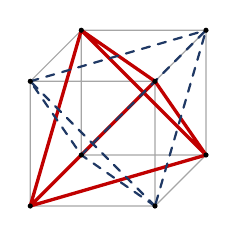
\begin{tikzpicture}[scale=0.72,line join=round,line cap=round,>=Stealth]
        \coordinate (A) at (0,0);     \coordinate (B) at (2.2,0);
        \coordinate (C) at (2.2,2.2); \coordinate (D) at (0,2.2);
        \coordinate (A') at (0.9,0.9);   \coordinate (B') at (3.1,0.9);
        \coordinate (C') at (3.1,3.1);   \coordinate (D') at (0.9,3.1);
        \draw[gray!70] (A)--(B)--(C)--(D)--cycle
                       (A')--(B')--(C')--(D')--cycle
                       (A)--(A') (B)--(B') (C)--(C') (D)--(D');
        \draw[accent,very thick] (A)--(C)--(B')--(D')--cycle (A)--(B') (C)--(D');
        \draw[ink,thick,dashed] (B)--(D)--(A')--(C')--cycle (B)--(A') (D)--(C');
        \foreach \p in {A,B,C,D,A',B',C',D'} \fill[black] (\p) circle (1.3pt);
      \end{tikzpicture}

      \footnotesize
      \raggedright
      顶点按坐标和奇偶分成两个正四面体（\textcolor{accent}{红} / \textcolor{ink}{蓝虚线}）。$O\cong S_4$ 的偶置换各自保持一个，奇置换交换两者，于是
      \[ \operatorname{Stab}(T_i)=A_4,\qquad [S_4:A_4]=2, \]
      这正是 $T\subset O$ 的几何来源。
    \end{column}
    \begin{column}{0.58\textwidth}
      \begin{block}{\footnotesize G204(a)：两个同构}
        \scriptsize
        $T\to S_4$：作用在 4 个顶点上，忠实。三阶旋转是 3-轮换、半转是双对换，都是偶置换，像落在 $A_4$；$|T|=12=|A_4|$，故 $T\cong A_4$。\\
        $O\to S_4$：作用在 4 条体对角线上，只有恒等固定全部 4 条，故忠实；$|O|=24=|S_4|$，故 $O\cong S_4$。
      \end{block}
      \begin{alertblock}{\footnotesize G200：$S_5$ 的正常子群只有 $1,A_5,S_5$}
        \scriptsize
        设 $1\ne N\trianglelefteq S_5$。则 $N\cap A_5\trianglelefteq A_5$，由 $A_5$ 单性只能取 $1$ 或 $A_5$。
        \begin{itemize}\setlength{\itemsep}{0pt}
          \item $N\cap A_5=A_5$：$A_5\subseteq N$，故 $N=A_5$ 或 $S_5$；
          \item $N\cap A_5=1$：符号映射限制在 $N$ 上单射，$|N|\le2$。若 $|N|=2$，$N$ 正规且 2 阶 $\Rightarrow N\subseteq Z(S_5)$，但 $Z(S_5)=1$，矛盾。故 $N=1$。
        \end{itemize}
        所以非平凡真正规子群只有 $A_5$。
      \end{alertblock}
    \end{column}
  \end{columns}
\end{frame}

% ============================================================ 22 G205-207
\begin{frame}[t]{六、\S7.4 精算 7/9：G205、G206、G207 三个"作用/中心"结论}
  \begin{columns}[T,onlytextwidth]
    \begin{column}{0.49\textwidth}
      \begin{exampleblock}{\footnotesize G205：$n>r!$ $\Rightarrow$ 有真正规子群}
        \scriptsize
        非平凡作用给出同态 $\varphi:G\to S_r$。
        \begin{itemize}\setlength{\itemsep}{0pt}
          \item $\ker\varphi\ne G$（作用非平凡）；
          \item 若 $\ker\varphi=1$，则 $G\le S_r$，$n=|G|\le r!$，与 $n>r!$ 矛盾。
        \end{itemize}
        故 $\ker\varphi$ 既真又非平凡，且核自动正规。
      \end{exampleblock}
      \begin{exampleblock}{\footnotesize G206：中心能有多大}
        \scriptsize
        (a) $Z(G)\subseteq Z(x)$ 且 $|Z(x)|=4$，由 Lagrange
        \[ |Z(G)|\mid4\ \Rightarrow\ |Z(G)|\in\{1,2,4\}. \]
        (b) $|C(y)|=4$ 即 $[G:Z(y)]=4$；由 $Z(G)\subseteq Z(y)$：
        \[ [G:Z(G)]=[G:Z(y)]\,[Z(y):Z(G)]=4\,[\cdots], \]
        故 $4\mid[G:Z(G)]$。（只能得到这个整除结论，不能定 $|Z(G)|$。）
      \end{exampleblock}
    \end{column}
    \begin{column}{0.49\textwidth}
      \begin{exampleblock}{\footnotesize G207：半素数阶中心化子交换}
        \scriptsize
        设 $C=Z(x)$，$|C|=pq$。因 $x$ 与 $C$ 中每个元素交换，
        \[ \langle x\rangle\subseteq Z(C). \]
        分两种：
        \begin{itemize}\setlength{\itemsep}{0pt}
          \item $|x|=pq$：$C=\langle x\rangle$，循环；
          \item $|x|=p$ 或 $q$：$[C:\langle x\rangle]$ 是素数，循环；$C/Z(C)$ 是它的商，也循环。
        \end{itemize}
        由引理 B（$G/Z$ 循环 $\Rightarrow$ 交换），$C$ 交换。
      \end{exampleblock}
      \footnotesize\color{ink!80}
      \starpt 三题各用一个工具：G205 用"核"，G206 用"包含链 + Lagrange"，G207 用"商群循环"。工具认得出来，题就一眼。
    \end{column}
  \end{columns}
\end{frame}

% ============================================================ 23 S_n 公式
\begin{frame}[t]{七、\S7.5 精算 1/4：轮换型的中心化子公式与两例}
  \begin{columns}[T,onlytextwidth]
    \begin{column}{0.49\textwidth}
      \begin{block}{\footnotesize 公式：$|Z(\sigma)|=\prod_k k^{m_k}m_k!$}
        \scriptsize
        设 $\sigma$ 的轮换型为 $1^{m_1}2^{m_2}\cdots n^{m_n}$。与 $\sigma$ 交换的置换必须把每个 $k$-轮换送到 $k$-轮换，选择分两步：
        \begin{enumerate}\setlength{\itemsep}{1pt}
          \item $m_k$ 个 $k$-轮换之间任意置换：$m_k!$ 种；
          \item 每个 $k$-轮换可独立旋转 $k$ 种：$k^{m_k}$ 种。
        \end{enumerate}
        故
        \[ Z(\sigma)\cong\prod_k\bigl(C_k\wr S_{m_k}\bigr),\qquad |Z(\sigma)|=\prod_k k^{m_k}m_k!, \]
        再由轨道--稳定化子得
        \[ |C(\sigma)|=n!\Big/|Z(\sigma)|. \]
      \end{block}
    \end{column}
    \begin{column}{0.49\textwidth}
      \begin{exampleblock}{\footnotesize G209：$S_5$ 中的 $(12)$}
        \scriptsize
        轮换型 $2\cdot1^3$：
        \[ |Z|=2^1\cdot1!\cdot1^3\cdot3!=2\cdot6=12, \]
        结构为 $C_2\times S_3$（$(12)$ 可转、其余 3 个点任意排），
        \[ |C|=120/12=10, \]
        即全部 10 个对换。
      \end{exampleblock}
      \begin{exampleblock}{\footnotesize G211：$S_7$ 中的 $(153)(246)$}
        \scriptsize
        轮换型 $3^2\cdot1$：
        \[ |Z|=3^2\cdot2!=18, \]
        结构为 $C_3\wr S_2=(C_3\times C_3)\rtimes C_2$（两个 3-轮换各自转，可整体交换），
        \[ |C|=7!/18=280. \]
      \end{exampleblock}
    \end{column}
  \end{columns}
\end{frame}

% ============================================================ 24 S7 阶 + G208(a)(b)
\begin{frame}[t]{七、\S7.5 精算 2/4：G210 $S_7$ 的元素阶 \& G208(a)(b)}
  \begin{columns}[T,onlytextwidth]
    \begin{column}{0.49\textwidth}
      \begin{block}{\footnotesize G210：元素阶 $=$ 分拆取 lcm}
        \scriptsize
        $S_7$ 的元素阶等于其轮换型各部分的最小公倍数。$7$ 的 15 个分拆只给出 9 个值：
        \begin{center}
          \renewcommand{\arraystretch}{1.1}
          \begin{tabular}{@{}c l@{}}
            \toprule
            阶 & 出现的轮换型（举例）\\
            \midrule
            $1$ & $1^7$\\
            $2$ & $2\cdot1^5$\\
            $3$ & $3\cdot1^4$\\
            $4$ & $4\cdot1^3$\\
            $5$ & $5\cdot1^2$\\
            $6$ & $3\cdot2\cdot1^2$\\
            $7$ & $7$\\
            $10$ & $5\cdot2$\\
            $12$ & $4\cdot3$\\
            \bottomrule
          \end{tabular}
        \end{center}
      \end{block}
    \end{column}
    \begin{column}{0.49\textwidth}
      \begin{block}{\footnotesize G208(a)：相邻对换生成一切对换}
        \scriptsize
        设 $i<j$，沿链"去而复返"：
        \[ (ij)=(i,i+1)(i+1,i+2)\cdots(j-1,j)\cdots(i+1,i+2)(i,i+1). \]
        中间的 $\cdots$ 是镜像回程，第二步到 $j$ 时已把 $i$ 送到 $j$，回程再把 $j$ 送回 $i$，中间点不动。于是所有对换都能写成相邻对换之积，而所有对换生成 $S_n$。
      \end{block}
      \begin{exampleblock}{\footnotesize G208(b)：长轮换要 $n-1$ 个，且不能更少}
        \scriptsize
        \[ (1\,2\cdots n)=(12)(23)\cdots(n-1,n). \]
        下界：设 $\tau$ 是任一置换，则 $\tau\cdot(j,j+1)$ 的轮换数（含不动点）与 $\tau$ 的轮换数相差 $1$。恒等有 $n$ 个轮换，长轮换只有 $1$ 个，故至少需要 $n-1$ 个对换。
      \end{exampleblock}
    \end{column}
  \end{columns}
\end{frame}

% ============================================================ 25 G208(c), Lang
\begin{frame}[t]{七、\S7.5 精算 3/4：G208(c) 与 Lang I.38 的其余小问}
  \begin{columns}[T,onlytextwidth]
    \begin{column}{0.49\textwidth}
      \begin{block}{\footnotesize G208(c) 与 Lang(a)：两种"少量生成元"}
        \scriptsize
        \textbf{长轮换 + 一个对换。} 设 $c=(1\,2\cdots n)$。共轭
        \[ c^{i-1}(12)c^{-(i-1)}=(i,i+1), \]
        得全部相邻对换，故 $c$ 与 $(12)$ 生成 $S_n$。\\
        \textbf{星形对换。} 对 $j>1$：
        \[ (1j)=(1,j-1)(j-1,j)(1,j-1), \]
        或用 $(ij)=(1i)(1j)(1i)$ 把任意对换写成星形的乘积，故 $(12),(13),\ldots,(1n)$ 生成 $S_n$。
      \end{block}
    \end{column}
    \begin{column}{0.49\textwidth}
      \begin{block}{\footnotesize Lang(d)：$n$ 素数 $+$ 任意一个对换就够}
        \scriptsize
        把字母看作 $\mathbb Z/n\mathbb Z$。$c^k(rs)c^{-k}=(k+r,\,k+s)$，所以能得到所有"差为 $d=s-r$"的对换。\\
        因 $n$ 素数且 $d\ne0$，$d$ 生成 $\mathbb Z/n\mathbb Z$，于是图
        \[ \bigl\{k,\ k+d\bigr\}\quad(k=0,\ldots,n-1) \]
        是连通的。\\
        \textbf{连通图引理：} 若图连通，取路径 $i=v_0,\ldots,v_m=j$，则
        \[ (v_0v_1)\cdots(v_{m-1}v_m)\cdots(v_0v_1)=(ij), \]
        故边上对换生成 $S_n$。于是 $c$ 与 $(rs)$ 生成 $S_n$。
      \end{block}
      \footnotesize\color{ink!80}
      \starpt 为什么必须 $n$ 素数：$n=6$、$d=2$ 时图分成两半，$c$ 与 $(13)$ 只生成一个真子群。
    \end{column}
  \end{columns}
\end{frame}

% ============================================================ 26 速查 A
\begin{frame}[t]{八、答案速查 A：\S7.2 八题 + \S7.3 前两题（12 题）}
  \centering
  \scriptsize
  \renewcommand{\arraystretch}{1.16}
  \setlength{\tabcolsep}{3pt}
  \begin{tabular}{@{}l l l c@{}}
    \toprule
    题号 & 题目 & 关键答案 / 结论 & 页\\
    \midrule
    LA198 & 5 个 $3\times3$ 矩阵的中心化子 & 对角 / 分块 / $aI+bN+cN^2$ / 中心对称；$A_3$：$ak\ne0$ & 6--7\\
    G125 & 至多 3 个共轭类 & $\{1\},C_2,C_3,S_3$；非交换只能是 $6=1+2+3$ & 8\\
    G126 & 5 阶正规 $N$ 必中心 & $G\to\operatorname{Aut}(C_5)$，像阶整除 $\gcd(|G|,4)=1$ & 5\\
    G127 & 类方程 $1+4+5+5+5$ & 阶 5 子群存在且正规；阶 4 存在但不正规 & 9\\
    LA199 & $SL_2(\mathbb F_3)$ 的类方程 & $24=1+1+4+4+4+4+6$；$U_1\nsim U_{-1}$（平方类） & 10\\
    G128 & 满射下的共轭类 & $\varphi(C)=C'$，$|C'|\mid|C|$（用 $\varphi^{-1}(Z_{G'})$） & 11\\
    G129 & $pq$ 阶必含 $p$ 阶元 & 反证；中心 $\ne1$ 用商群，中心 $=1$ 得 $pq=1+kp$ 矛盾 & 11\\
    LA200 & $A_d$ 与 $B_d$ 何时共轭 & $GL_2$ 恒共轭；$SL_2\iff |d|>2$（二次型不定） & 12\\
    G195 & 不动点定理 & $|S|\equiv|S^G|\pmod p$；$p\nmid|S|\Rightarrow S^G\ne\varnothing$ & 13\\
    G196 & $G/Z(G)$ 循环 $\Rightarrow$ 交换 & 元素写成 $a^m z$，中心元可交换 & 5\\
    G197 & 非交换 $p^3$ & $|Z|=p$，$|Z(x)|=p^2$，$p^3=p+(p^2-1)p$ & 14\\
    G198 & 8 阶群分类 & $C_8,\,C_4\times C_2,\,C_2^3,\,D_4,\,Q_8$；后两个用元素阶分开 & 15\\
    \bottomrule
  \end{tabular}
\end{frame}

% ============================================================ 27 速查 B
\begin{frame}[t]{八、答案速查 B：\S7.4 九题 + \S7.5 四题（13 题）}
  \centering
  \scriptsize
  \renewcommand{\arraystretch}{1.16}
  \setlength{\tabcolsep}{3pt}
  \begin{tabular}{@{}l l l c@{}}
    \toprule
    题号 & 题目 & 关键答案 / 结论 & 页\\
    \midrule
    G199 & 内接立方体的稳定化子 & $60/5=12\cong T\cong A_4$（$I$ 在 5 个立方体上传递） & 20\\
    G200 & $S_5$ 的正常子群 & 只有 $1,A_5,S_5$；$N\cap A_5\in\{1,A_5\}$，$A_5$ 单 & 21\\
    G201 & $I$ 中对合的中心化子 & $60/15=4\cong V_4$（15 个对合全共轭） & 20\\
    G202 & $T$ 的类方程 & $12=1+3+4+4$；$V_4$ 正规；无 6 阶子群 & 17\\
    G203 & $O$ 的类方程 & $24=1+6+3+8+6$；真正规子群 $V_4,A_4$ & 18\\
    G204 & $T\cong A_4$，$O\cong S_4$ & 4 顶点 / 4 体对角线；$A_4\subset S_4$ 由双内接四面体实现 & 21\\
    G205 & $n>r!$ 必有真正规子群 & 核 $\ker\varphi$ 既真又非平凡 & 22\\
    G206 & 中心的大小 & $|Z(x)|=4\Rightarrow|Z(G)|\in\{1,2,4\}$；$|C(y)|=4\Rightarrow4\mid[G:Z(G)]$ & 22\\
    G207 & $|Z(x)|=pq$ $\Rightarrow$ 交换 & $C/\langle x\rangle$ 循环，$C/Z(C)$ 是它的商，用引理 B & 22\\
    G208 & $S_n$ 的生成元 & 相邻对换；长轮换 $n-1$ 个且最少；$c+(12)$；$n$ 素数 $+$ 任意对换 & 24--25\\
    G209 & $S_5$ 中 $(12)$ 的中心化子 & $C_2\times S_3$，$|Z|=12$，类大小 10 & 23\\
    G210 & $S_7$ 的元素阶 & $1,2,3,4,5,6,7,10,12$（分拆取 lcm） & 24\\
    G211 & $S_7$ 中 $(153)(246)$ & $C_3\wr S_2$，$|Z|=18$，$|C|=280$ & 23\\
    \bottomrule
  \end{tabular}
\end{frame}

% ============================================================ 28 方法卡
\begin{frame}[t]{九、六张方法卡：看到什么，用哪一招}
  \begin{columns}[T,onlytextwidth]
    \begin{column}{0.325\textwidth}
      \begin{block}{\footnotesize 1. 问"类多大"}
        \scriptsize 用 $|C(x)|=[G:Z_G(x)]$ 双向换算。给中心化子尺寸、给类大小、给指数，三者是一回事。\par\vspace{1pt}
      \end{block}
      \begin{block}{\footnotesize 2. 找正规子群}
        \scriptsize 先写类方程，再枚举"含 $1$ 的类之和"，只留整除 $|G|$ 的。\par\vspace{1pt}
      \end{block}
    \end{column}
    \begin{column}{0.325\textwidth}
      \begin{block}{\footnotesize 3. 正规 $\Rightarrow$ 作用到 $\operatorname{Aut}$}
        \scriptsize $G\to\operatorname{Aut}(N)$；$|\operatorname{Aut}(N)|$ 与 $|G|$ 互素 $\Rightarrow$ 像平凡 $\Rightarrow N$ 中心。\par\vspace{1pt}
      \end{block}
      \begin{block}{\footnotesize 4. 商群循环 $\Rightarrow$ 交换}
        \scriptsize 要排除 "$|Z|$ 太大"或证明某个子群交换时，先看 $G/Z(G)$ 是否循环。\par\vspace{1pt}
      \end{block}
    \end{column}
    \begin{column}{0.325\textwidth}
      \begin{block}{\footnotesize 5. $p$-群用不动点}
        \scriptsize $|S|\equiv|S^G|\pmod p$；共轭作用给 $|Z|\equiv|G|\pmod p$，先把中心撑起来。\par\vspace{1pt}
      \end{block}
      \begin{block}{\footnotesize 6. 作用 $\Rightarrow$ 同态}
        \scriptsize 非平凡作用给 $G\to S_r$，核自动正规（G205）；轨道大小 $=[G:G_s]$ 算稳定化子阶（G199/G201）。\par\vspace{1pt}
      \end{block}
    \end{column}
  \end{columns}
  \vspace{0.15em}
  \begin{exampleblock}{\footnotesize 这套组合拳在本周的覆盖面}
    \scriptsize
    25 题里，8 题"套公式直接算"（类大小、中心化子、元素阶）；11 题"用整除性排除"（类方程拼正规子群、$|Z|$ 的可能值、$|d|>2$、$pq=1+kp$）；6 题"同态核或商群的一次应用"（G126、G196、G205、G207、G128、G208 的生成元论证）。
  \end{exampleblock}
\end{frame}

% ============================================================ 29 易错点
\begin{frame}[t]{十、易错点与来源问题（都能在笔记里回查）}
  \begin{columns}[T,onlytextwidth]
    \begin{column}{0.49\textwidth}
      \begin{alertblock}{\footnotesize LA200：题面维度不一致}
        \scriptsize
        矩阵是 $2\times2$，环境群印成 $GL_n(\mathbb R),SL_n(\mathbb R)$。笔记保留原题并标 \texttt{Source issue}，按 $n=2$ 求解；不要悄悄改题面。
      \end{alertblock}
      \begin{alertblock}{\footnotesize G200："proper" 的字面陷阱}
        \scriptsize
        字面含平凡子群，答案"否"；本意"非平凡真"，此时 $A_5$ 唯一。两种读法都要交代。
      \end{alertblock}
      \begin{alertblock}{\footnotesize LA199：$GL$ 与 $SL$ 的类不同}
        \scriptsize
        共轭只能把幂零项乘上 $\lambda^2$；$\mathbb F_3^\times$ 的非零平方只有 $1$，所以 $U_1\nsim U_{-1}$。换到 $GL_2$ 才合并成一类。
      \end{alertblock}
    \end{column}
    \begin{column}{0.49\textwidth}
      \begin{alertblock}{\footnotesize G208：下界与构造要分开写}
        \scriptsize
        写出 $n-1$ 个乘积只证"$\le n-1$"；必须补"每个对换至多改变一个轮换数"才能说最少。
      \end{alertblock}
      \begin{alertblock}{\footnotesize G195：只保证"至少一个"}
        \scriptsize
        $p\nmid|S|$ 时只能断言 $S^G\ne\varnothing$；不能推出 $|S^G|>1$，也不能反推别的轨道大小。
      \end{alertblock}
      \begin{alertblock}{\footnotesize 类方程相同 $\ne$ 同构}
        \scriptsize
        $D_4$ 与 $Q_8$ 的类方程、中心阶都相同；必须再用元素阶剖面或子群结构区分。这是本周唯一一处"类方程不够用"。
      \end{alertblock}
      \begin{alertblock}{\footnotesize 记号：$Z(G)$ 与 $Z(x)$}
        \scriptsize
        $Z(G)=\bigcap_x Z(x)$ 是中心；类大小公式里永远是 $Z(x)$，"$N$ 中心"才用 $Z(G)$。
      \end{alertblock}
    \end{column}
  \end{columns}
\end{frame}

% ============================================================ 30 收尾
\begin{frame}[t]{十一、收尾：数据、自测 8 题、明天的动作}
  \begin{columns}[T,onlytextwidth]
    \begin{column}{0.55\textwidth}
      \begin{block}{\footnotesize 讲完当场自测（先盖住答案）}
        \scriptsize
        \begin{enumerate}\setlength{\itemsep}{1pt}
          \item $|Z_{S_5}((12))|$ 是多少？为什么不是 $60/10$？
          \item $D_4$ 与 $Q_8$ 类方程相同，用什么区分？
          \item 证明：$|N|=5$、$N\trianglelefteq G$、$|G|$ 奇 $\Rightarrow N\subseteq Z(G)$；把"奇"去掉给一个反例。
          \item $U_1$ 与 $U_{-1}$ 在 $SL_2(\mathbb F_3)$ 中共轭吗？为什么？
          \item 写出非交换 $p^3$ 的类方程，并用 $p=2$ 与 $D_4$ 对账。
          \item $A_4$ 为什么没有 6 阶子群？
          \item $I$ 中一个对合的中心化子阶与结构？
          \item $(1\,2\cdots n)$ 最少用几个对换？证明下界。
        \end{enumerate}
        答案位置：第 23、15、5、10、14、17、20、24 页。
      \end{block}
    \end{column}
    \begin{column}{0.43\textwidth}
      \begin{exampleblock}{\footnotesize 明天之后的两件事}
        \scriptsize
        \begin{itemize}\setlength{\itemsep}{2pt}
          \item \textbf{补 Random Review}：本周 6 份清单全空。抽 \ex{G203}、\ex{LA200}、\ex{G211} 三条，正好覆盖"类方程 / 矩阵共轭 / 轮换型"。
          \item \textbf{接续 \S7.5}：明天清单从 5.5 题起；若 10-18 的 3 题要一起讲，按 \S7.5 结构补一页、速查表补一行、页码顺延。
        \end{itemize}
      \end{exampleblock}
      \begin{block}{\footnotesize 本周数字}
        \scriptsize
        \begin{tabular}{@{}ll@{}}
          清单 & 6 份（10-12 -- 10-17）\\
          题目 & 25 道（群论 22、线代 3）\\
          难度 & 入门 6 / 中等 11 / 高级 8\\
          含 Lang 交叉题 & 2 道（G198、G208）\\
          Random Review & 0 条\\
        \end{tabular}
      \end{block}
    \end{column}
  \end{columns}
  \vspace{0.2em}
  {\scriptsize\color{ink!70} 一句话：本周 25 题最终都落在三个量上——$|G|$、$|Z(x)|$、$|C(x)|$；把"群的结构问题"换成"整除性与类之和"，就是这一章的通行证。}
\end{frame}

\end{document}
